% Small intro, re-explain that finding thread/core pairing is complicated and thus ML is a good idea.

\begin{figure}[t]
  \centering
 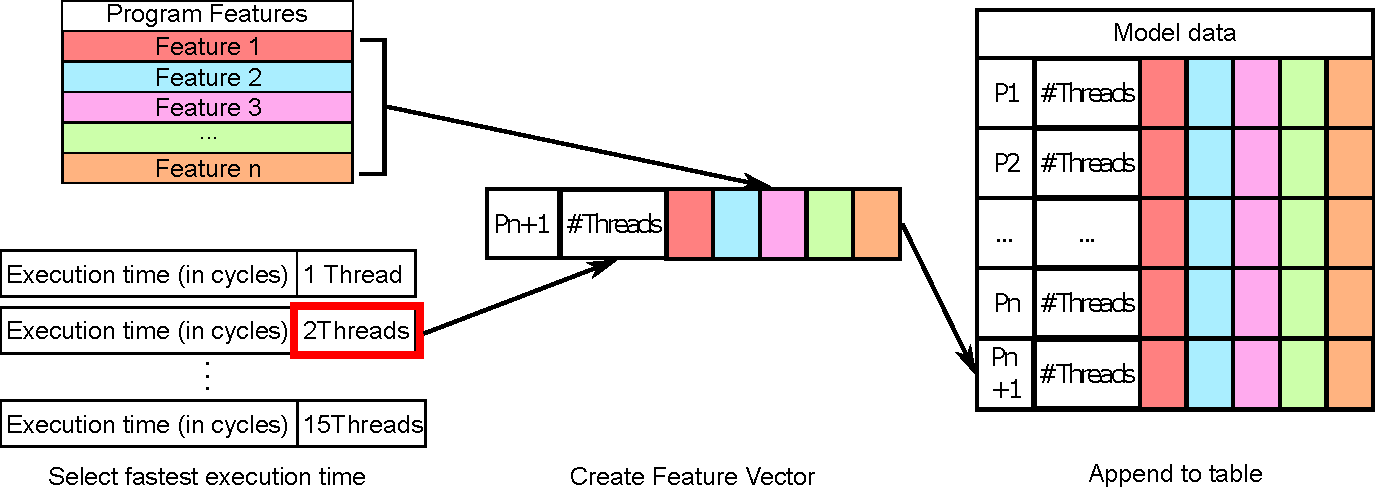
\includegraphics[width=1\textwidth]{streamit-paper/graphics/thread_expl.pdf}
  \caption{Visual representation of how data was collected for the threading model.}\label{fig:thread_expl}
\end{figure}
As seen in the previous section, selecting the right number of threads and a good combination of cores is difficult.
This difficulty arises from trying to balance between exploiting instruction level parallelism (ILP) by composing a large amount of cores and exploiting TLP by generating more threads.
As the design space is large, it is important to automate the decision making to alleviate the task of getting the best performance out of the streaming application at hand.
The problem of automating this decision can be decomposed into two stages; first, determining the right number of threads and second, selecting a good core composition.
Partitioning the program is done first as it is more natural to split the program up into threads before determining how many cores each thread requires.
In this section, two machine-learning models that predict the best thread partitioning and core composition to maximise performance are presented.

\subsection{Predicting the number of threads}
\subsubsection{Correlation Analysis}
%In this section, when discussing correlation we specifically look at which variables correlate with the optimal number of threads.

To build the threading model, the synthetic benchmarks previously described in~\ref{chp:stream:sec:setup} are used.
Figure~\ref{fig:thread_expl} shows the overview of how the data for the model is collected.
For each of the synthetic benchmark 15 different threaded versions are generated and assigned a single core per thread.
They are then all executed and their cycle count is recorded; this is repeated for 1000 unique synthetic applications. 
Once all the data is generated, the number of threads that leads to the fastest execution time is saved to a table with a set of features that define the program.

In order to build the two machine learning models an initial set of over 50 features are extracted from StreamIt programs.
These features are extracted using pre-existing analytical tools within StreamIt and some counters added specifically for this chapter.
As some of the 50 features may not contain any valuable information, the features selected for the models are determined through correlation analysis.
The highest correlating features are used by the model to make a prediction about the number of threads to use.
Figure~\ref{fig:corr} shows the 10 variables that correlate the most with determining the optimal thread number.
It is important to note that these features all correlate positively with the number of threads the program requires to get the fastest execution time.
In StreamIt the term \textit{multiplicity} defines the number of times a filter will have to execute in a time slice when the graph is in a steady state~\cite{gordon2002streamcomp}.

\begin{figure}[t]
  \centering
 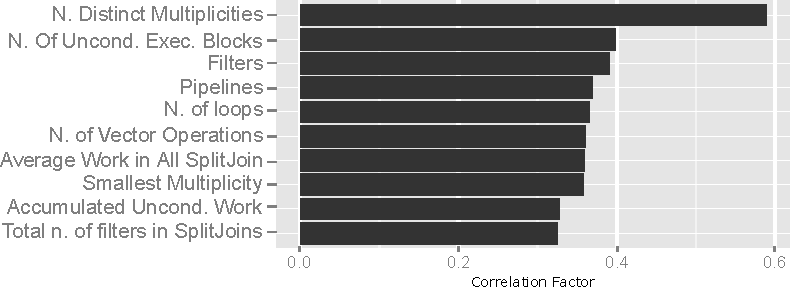
\includegraphics[width=1\textwidth]{streamit-paper/graphics/corrThreadRemix2.pdf}
  \caption{The ten highest correlating features with the best number of threads for 1000 synthetic benchmarks.}\label{fig:corr}
  \vspace{-1em}
\end{figure}
 
The 10 features can be described as followed:
\begin{itemize}
\item Number of Distinct Multiplicities: the variety of different execution rates of filters per time slice.
\vspace{-0.5em}
\item Number of unconditionally executed blocks: amount of operations in a filter that always execute.
\vspace{-0.5em}
\item Filters: number of filters found in the benchmark.
\vspace{-0.5em}
\item Pipelines: number of pipelines found in the benchmark.
\vspace{-0.5em}
\item Number of Loops: amount of loops present in the benchmark.
\vspace{-0.5em}
\item Number of Vector Operations: amount of potential vector operations found in the benchmark.
\vspace{-0.5em}
\item Average Work in all SplitJoins: average amount of operations per SplitJoin.
\vspace{-0.5em}
\item Smallest Multiplicity: The smallest execution rate of a single filter.
\vspace{-0.5em}
\item Accumulated Unconditional Work: Total number of operations in all filters which must be executed.
\vspace{-0.5em}
\item Total Number of filters in SplitJoins: Amount of filters that are found in SplitJoins.
\end{itemize}

According to Figure~\ref{fig:corr} the highest correlating value is Number of Distinct Multiplicities found in the StreamIt application.
There are very little variables that highly correlate beyond Number of Distinct Multiplicities.
A high number of distinct multiplicities implies that the StreamIt application features an important amount of filters with different execution rates.
This means that certain filters may be local bottlenecks in a Pipeline for example.
Multithreading the pipelines with local bottlenecks will help alleviate the problem of multiple distinct multiplicities as it can isolate the filters with longer firing rates to allow smaller filters to execute more often.

For example, the benchmark \bench{ChannelVocoder} only has 66\% of its filters sharing the same average multiplicity of 50~\cite{thiesStreamit2010}, with a minimum multiplicity of 1. 
The benchmark features a single SplitJoin yet when recalling section \ref{sec:streamit:dse}'s Figure~\ref{fig:overviewhist} \bench{ChannelVocoder}'s performance is greatly improved via multi-threading.
The number of threads also depends on certain structural features such as Pipelines, SplitJoins and number of Filters.
Yet, these variables seem to hold less influence on the number of threads a program needs than the different multiplicities found in the graph.
This is most certainly due to the fact that whilst SplitJoins make parallelisable areas more visible, if there is very little work in each stream, increasing the number of threads will make performance worse as it increases the communication to comptuation ratio.

It is also important to understand that a high number of Pipelines implies the use of SplitJoins.
This is due to the fact that a StreamIt application with no SplitJoins will feature only a single Pipeline, thus a larger number of pipelines implies at least one SplitJoin.
This is why the number of SplitJoins is not present in the correlating features; because the number of Pipeline already correlates with this feature.\\

A method of determining how many threads an application requires is to build a database of programs.
Each entry in the database contains a feature vector for a program and the number of threads that leads to the best performance.
When a new program is encountered, the database can be searched to find applications that have similar features to determine the number of threads needed.
To implement such a model, k-Nearest Neighbor (kNN) is deployed.
As programs will most likely not have the same values for each feature, using kNN allows to estimate the thread count by comparing the feature vector of an unknown program with a group of known programs.
Given a new application, the classifier determines the $k$ closest synthetic applications.
The distance between the features is measured using the Euclidean distance for each application.
Once the set of $k$ nearest neighbors is identified, the model averages the best number of threads for each of the neighbors to make a prediction. 
The parameter $k$ was determined experimentally using only the synthetic benchmarks.
A value of $k=7$ was found to lead to the best performance.
The features chosen are the ten variables displayed in Figure~\ref{fig:corr}.

%\begin{table}[t]
% The FFT need are variable
%  \small
% \begin{tabular} { | l | l | l | }
% \hline
% \cellcolor[gray]{0.7}Distance from best thread count  & \cellcolor[gray]{0.7} Accuracy of kNN &  \cellcolor[gray]{0.7} Performance Penanlty\\ \hline
%  0 & 33\% & 0\\ \hline
%+/- 1 & 57\% & 12\\ \hline
%+/- 2 & 67\% & 19\\\hline

 %\end{tabular}
 % \caption{Performance of kNN model.}\label{tab:instancefilt}
%\end{table}
%\subsubsection{kNN Model}
%\paragraph*{Validating the model.}
%Cross validation is used to determine the efficiency of the model by observing how close a classification is to the measured best thread number.
%It involves validating all the points in the training data by removing them from the model, more details can be found in Chapter~\ref{chp:Background}.
%Using cross validation the model generated in this chapter has a 33\% accuracy of getting the exact best thread number.
%The accuracy increases to 57\% when allowing a prediction to be 1 thread away from the best and 67\% when 2 threads away.
%On average, having a thread number that is +/- 1 away from the optimal thread count only incurrs a 12\% performance penalty.
%For a distance of +/- 2 this increases to 19\%.
%This penalty was measured by comparing the performances of the synethtic benchmarks using only multithreading.
%With this in mind, it is important to understand that accuracy is not the final metric that is used to evaluate the model.
%Instead, what does matter is the performance of the application when using the configuration predicted by both the thread and core predictor, which is discussed in section~\ref{sec:results}.

